\chapter{Results}
This chapter present the results of the bachelor thesis. Modifications which influence the structure of the program and the behavior of the simulation are presented at the beginning. Later the results of the desired cell as a sphere as well as the result of the created algorithm are revealed. In the last section evaluations of 3D simulations are shown.

\section{Structure of the program}
With the removement of unessesary methods and variables, which are not used, the program becomes more readable and is easier to understand. These changes decrease the probability of errors and confusion during code analysis, i.e. studying of the code. By declaring abstract methods the program becomes more structured. Because identical methods are not written again in classes which inherit from each other it is easier to understand the program as well to find errors. \newline
The changes of section \ref{sec:LambdaMultipliers} and \ref{sec:AbstractMethods} modify the program in a way that it is more structured and understandable. This improves the time required for the code analysis, which is important for newcomers to the project, as well as to find errors. 

\section{Improvements of the program}
During the bachelor thesis several adjustments in the program were made. All these changes are important for the simulation as they effect the simulation. These changes were tested by using the output command to see the required information at the command line. 
\subsection{Calculation of the amount of stem cells on the basal membrane}
With the changes of section \ref{sec:AmountStemCellsBasalMembrane} the program now has a calculation of the amount of stem cells on the basal membrane for two and three dimensions. The new calculation is correct for every simulation size in 2D and 3D. This is important as the program should be able to have a correct implementation for two as well as for three dimensions. An example at the initialization of a simulation is displayed in figure \ref{img:SimulationAtMCS0} at page \pageref{img:SimulationAtMCS0}.
\subsection{\ac{MCS} until the urination event}
Because the calculation until the urination event was modified in section \ref{sec:calculationStpesUntilUrination} the urination now takes place every six hours instead of every twelf hours. This change is important for the simulation because with an urination every twelf hours the simulation is not as real as with the event every six hours. Moreover, in the paper \cite{Torelli2017} of the project it is written that this event occurs every six hours. This change helps the simulation to not only be more realistic it is also important in order that there are not too many cells in the simulation field. As a result of too many cells in the simulation field the simulation stops. Thus, the change increases the reality and helps to prevent an overflow of cells.
\subsection{Target volume and target surface after mitosis}
The modification of section \ref{sec:TargetVolumeSurfaceAfterMitosis} effects the simulation in a way that after mitosis both cells are able to grow immediately. Without the modification the cell with a too small target volume and target surface would not growth several calculation steps. Therefore, the cell does not grow several calculation steps until the target volume becomes larger than the current volume. Because the target volume of both created cells is now set dependent of the by \ac{CC3D} given volume of each cell, it is not possible that one of the two cells has a smaller target volume and surface than the current volume and surface. With this modification both cells, created during mitosis, are now able to grow immediately.
\subsection{Convertion between physical unit and the voxel unit}
The simulation is effected in a positive way because of the changes of section \ref{sec:ApproximationError}. The modifications in this section are crucial since now the calculation of volume constraints of each cell type is more precise. With this modification every convertion of \SI{}{\micro\metre} into pixels and voxels is now free of calculation errors. Because the result of the calculations of the volume constraints of the different cell types is used to determine when mitosis takes place it is important to have them without an calculation error. Because the result is converted only at the end, simulations beside a voxel density of 1 have also the correct volume constraints of the cells. Moreover, this calculation is also used to calculate the growth per calculation step in the simulation, since the growth of a cell is calculated in the physical unit and then converted into pixels. Because the calculation of the volume constraints of the different cell types and the calculation of the growth of each cell each \ac{MCS} are two major parts of the simulation, this modification is important and effects the correctness of simulations.
\newline
\newline

\begin{figure}[ht]
	\center
	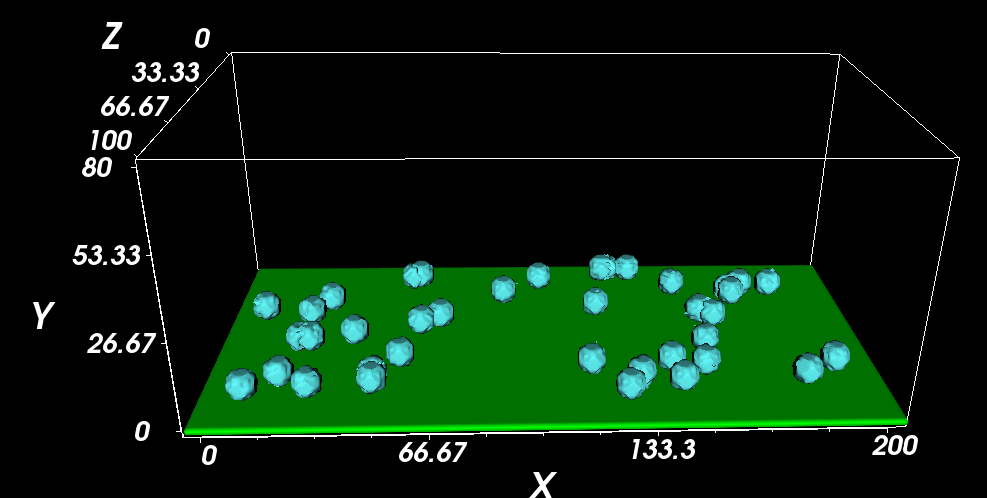
\includegraphics[scale=0.4]{figures/SimulationAtMCS0.png}
	\caption[Spread stem cells at the basal membrane at \ac{MCS} 0]{Spread stem cells at the basal membrane at \ac{MCS} 0. The box displays the simulation field, with a size of \SI{100}{\micro\metre} at the x-asis, \SI{80}{\micro\metre} at the y-axis and \SI{100}{\micro\metre} at the z-axis. In the simulation the green bottom displays the basal membrane and at the basal membrane the stem cells are spread. The amount of these stem cells is calculated as in section \ref{sec:AmountStemCellsBasalMembrane} explained.}
	\label{img:SimulationAtMCS0}
\end{figure}


\section{Draw sphere cells}
With the created method of section \ref{sec:DrawSphereCells} the program is now able to draw a sphere cell, as it is displayed in figure \ref{img:DrawnSphereCellRadius5And9} and \ref{img:DrawnSphereCellRadius14And23} at page \pageref{img:DrawnSphereCellRadius5And9} and page \pageref{img:DrawnSphereCellRadius14And23}. \newline
Since voxels, cuboids, are used in the 3D simulation to draw a sphere cell, it is not possible to draw a perfectly round sphere. This problem is displayed with an circle and a square in picture \ref{img:CircleSquarePixels} at page \pageref{img:CircleSquarePixels}, since the circle and square are the 2D objects of an sphere and cuboid. The drawn cells are as spherish as possible in the simulation with the use of voxels. \newline
Figure \ref{img:DrawnSphereCellRadius5And9} displays two independent drawn cells with a radius of \SI{5}{\micro\metre} and \SI{9}{\micro\metre}. These cells show that there are a lot of edges in the sphere. As the radius increases, the sphere shape of the cell gets more detailed, as it is displayed in figure \ref{img:DrawnSphereCellRadius14And23}. In figure \ref{img:DrawnSphereCellRadius14And23} two cells are drawn idepently with a radius of \SI{14}{\micro\metre} and \SI{23}{\micro\metre}. With the increase of the radius, the deviation of the surface increases as well, as it is shown in figure \ref{img:DeviationSphere} at page \pageref{img:DeviationSphere}. This might be a result as the surface of a sphere and a cuboid, with the daimeter $2 \cdot r$, deviates more as $r$ increases.

\begin{figure}[ht]
	\begin{center}
	\subfloat[]{
		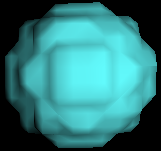
\includegraphics[scale=1.05]{figures/VoxelSphere/Radius5-0.png}
	}
	\subfloat[]{
		\hspace{0.5cm}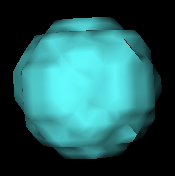
\includegraphics[scale=1.05]{figures/VoxelSphere/Radius5-1.png}
	}
	\end{center}
	\begin{center}
	\subfloat[]{
		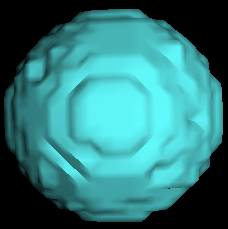
\includegraphics[scale=0.74]{figures/VoxelSphere/Radius9-0.png}
	}
	\subfloat[]{
		\hspace{0.5cm}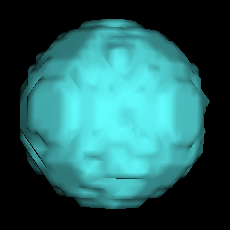
\includegraphics[scale=0.735]{figures/VoxelSphere/Radius9-1.png}
	}
	\end{center}
	\caption[Drawn sphere cells with a radius of 5 and 9]{\label{img:DrawnSphereCellRadius5And9}A single cell drawn into the simulation field. The radius of the cell of (a) and (b) is 5 and the radius of the cell of (c) and (d) is 9. Pictures (a) and (c) are with the front view, whereas the
pictures (b) and (d) have an view angle of around 45 degree. The color of the cell is chosen in
a way that more details are visible.}
\end{figure}

\begin{figure}[ht]
	\begin{center}
	\subfloat[]{
		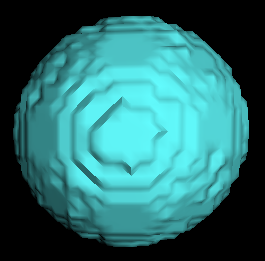
\includegraphics[scale=0.65]{figures/VoxelSphere/Radius14-0.png}
	}
	\subfloat[]{
		\hspace{0.5cm}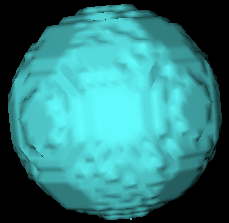
\includegraphics[scale=0.76]{figures/VoxelSphere/Radius14-1.png}
	}
	\end{center}
	\begin{center}
	\subfloat[]{
		\hspace{0.1cm}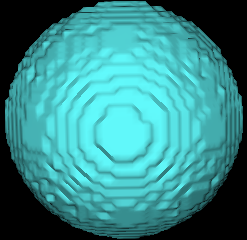
\includegraphics[scale=0.705]{figures/VoxelSphere/Radius23-0.png}
	}
	\subfloat[]{
		\hspace{0.5cm}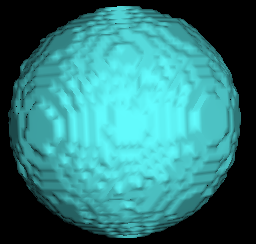
\includegraphics[scale=0.695]{figures/VoxelSphere/Radius23-1.png}
	}
	\end{center}
	\caption[Drawn sphere cells with a radius of 14 and 23]{\label{img:DrawnSphereCellRadius14And23}A single cell drawn into the simulation field. The radius of the cell of (a) and (b) is 14 and the radius of the cell of (c) and (d) is 23. Pictures (a) and (c) are with the front view, whereas the
pictures (b) and (d) have an view angle of around 45 degree. The color of the cell is chosen in
a way that more details are visible.}
\end{figure}


\section{Calulate the voxel volume and surface sites of a sphere cell}
The created algorithm of section \ref{sec:CreatedAlgorithm} is able to calculate out of a given radius the volume, of a sphere cell created with cuboids, in voxel as well as it is able to count the surface sites of the cell. Moreover, it is also possible to calculate the physical volume and surface of a sphere with a given radius. With this algorithm it is possible to calculate the volume and surface of a sphere cell and become the same result as \ac{CC3D} calculates. \newline
The algorithm is useful but also has its weaknesses. For a voxel density beside 1 the results between the created algorithm and \ac{CC3D} deviate. The results differ also if the radius is not a whole number. There are no insights how \ac{CC3D} calculates the volume and surface of a drawn sphere cell. Moreover, for the tenths part of five to nine of the radius, for every radius between $.5$ until $.9$, it is possible to create the cube with an radius which is either rounded up or down. This means for a radius of $3.7$ it is possible to use either six or eight voxels to create the cuboid. Seven voxels are not possible because then the sphere would loose its symetry. \newline
The algorithm helps to calculate the volume of a sphere cell, out of voxels, as well as to count the surface sites. It is able to be executed without an start of an simulaion. Thus, there is no need to adjust the coding of the project and to wait until the simulation started to recieve the volume and surface values of a sphere cell. 

\section{Grow sphere cells}
In section \ref{sec:GrowSphereCell} the factor for the calculation of the surface of the cell was evidenced best to be $1.5$ for a voxel density of 1. With this factor it should be possible to let the sphere cell grow as a sphere. To test the growth of the cell, one single cell was placed in the simulation field. As the cell growed during the simulation the volume and surface values were rad out of the command line and compared to the documented values of a drawn cell. \newline
To let a cell grow as a sphere does not work. Even the volume and surface values, calculated by \ac{CC3D}, and the target volume and target surface values, calculated by the program, meet the values of sphere cells with a small deviation of an maximum deviation up to 50 voxels. \newline
In figure \ref{img:GrowthSphereCellRadius5} and \ref{img:GrowthSphereCellRadius9} at page \pageref{img:GrowthSphereCellRadius5} and \pageref{img:GrowthSphereCellRadius9} examples of the growth of two stem cells with a different radius are displayed. It is observable that these cells are not able to keep the shape with which they were depicted.


\begin{figure}[ht]
	\begin{center}
	\subfloat[]{
		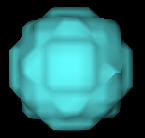
\includegraphics[scale=1.15]{figures/GrowthSphereCell/Radius5/Radius5-MCS0.png}
	}
	\subfloat[]{
		\hspace{0.5cm}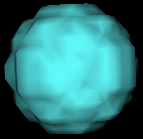
\includegraphics[scale=1.142]{figures/GrowthSphereCell/Radius5/Radius5-MCS0-1.png}
	}
	\end{center}
	\begin{center}
	\subfloat[]{
		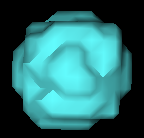
\includegraphics[scale=1.16]{figures/GrowthSphereCell/Radius5/Radius5-MCS50.png}
	}
	\subfloat[]{
		\hspace{0.5cm}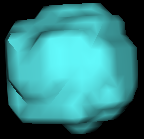
\includegraphics[scale=1.155]{figures/GrowthSphereCell/Radius5/Radius5-MCS50-1.png}
	}
	\end{center}
	\begin{center}
	\subfloat[]{
		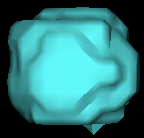
\includegraphics[scale=1.145]{figures/GrowthSphereCell/Radius5/Radius5-MCS250.png}
	}
	\subfloat[]{
		\hspace{0.53cm}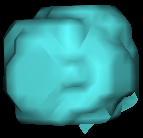
\includegraphics[scale=1.145]{figures/GrowthSphereCell/Radius5/Radius5-MCS250-1.png}
	}
	\end{center}
	\caption[Growth of a sphere cell with a radius of 5]{\label{img:GrowthSphereCellRadius5}A sphere cell, with a radius of \SI{5}{\micro\metre} and a voxel density of 1, as it grows. Images (a), (c) and (e) are the front view of the cell and figures (b), (d) and(f) have around a 45 degree angle of the front. Figure (a) and (b) are at \ac{MCS} 0, images (c) and (d) at calculation step 50 and figures (e) and (f) present \ac{MCS} 250.}
\end{figure}

\begin{figure}[ht]
	\begin{center}
	\subfloat[]{
		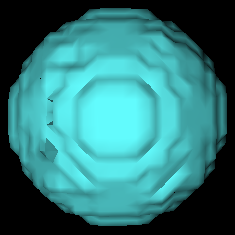
\includegraphics[scale=0.7]{figures/GrowthSphereCell/Radius9/Radius9-MCS0.png}
	}
	\subfloat[]{
		\hspace{0.5cm}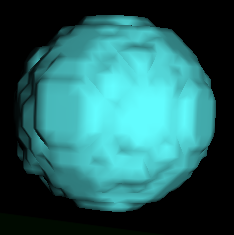
\includegraphics[scale=0.7]{figures/GrowthSphereCell/Radius9/Radius9-MCS0-1.png}
	}
	\end{center}
	\begin{center}
	\subfloat[]{
		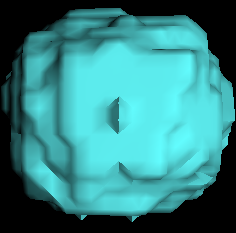
\includegraphics[scale=0.7]{figures/GrowthSphereCell/Radius9/Radius9-MCS250.png}
	}
	\subfloat[]{
		\hspace{0.5cm}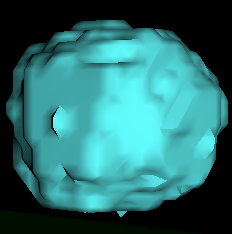
\includegraphics[scale=0.698]{figures/GrowthSphereCell/Radius9/Radius9-MCS250-1.png}
	}
	\end{center}
	\begin{center}
	\subfloat[]{
		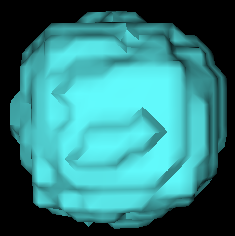
\includegraphics[scale=0.7]{figures/GrowthSphereCell/Radius9/Radius9-MCS750.png}
	}
	\subfloat[]{
		\hspace{0.5cm}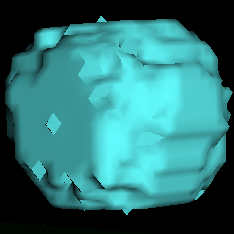
\includegraphics[scale=0.7]{figures/GrowthSphereCell/Radius9/Radius9-MCS750-1.png}
	}
	\end{center}
	\caption[Growth of a sphere cell with a radius of 9]{\label{img:GrowthSphereCellRadius9}A sphere cell, with a radius of \SI{9}{\micro\metre} and a voxel density of 1, as it grows. Images (a), (c) and (e) are the front view of the cell and figures (b), (d) and(f) have around a 45 degree angle of the front. Figure (a) and (b) are at \ac{MCS} 0, images (c) and (d) at calculation step 250 and figures (e) and (f) present \ac{MCS} 750.}
\end{figure}


\section{Adhesion}
The new adhesion matrix is different than the one which was used until this thesis. Out of the observations of section \ref{sec:AdhesionMatrix} the new adhesion matrix was created. The matrix is displayed in table \ref{tbl:NewAdhesion}. The values were chosen in a way that cells of one layer stick to each other and try to increase the area where the cells touch. The adhesion for cells at one layer was observed not to be too high in order that the cells do not infiltrate each other. An example therefore is displayed in figure \ref{img:InfiltratingCells} at page \pageref{img:InfiltratingCells}. If cells infiltrate each other it is a sign of too high adhesion energy. For the adhesion between cells of different layers in the urothelium the values were chosen in a way that the cells connect with each other but that they grow independent. It is important that the cells of different layers do not connect to strong to each other, otherwise the different layers in the urothelium might be mixed. 
\begin{figure}[ht]
	\center
	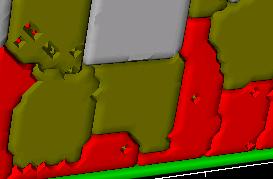
\includegraphics[scale=1.2]{figures/TooHighAdhesion1.png}
	\caption[Different cells try to infiltrate each other]{Different cells try to infiltrate each other as a reason of too high adhesion values between the cells. The different points at the surface of a cell are an indicator that a surrunding cell tries to infiltrate the cell at which the points occur.}
	\label{img:InfiltratingCells}
\end{figure}


\begin{table}[ht]
\centering
\caption[New adhesion values for the different cell types]{New adhesion values for the adhesion between the different cell types. M, the medium cell type, is a of \ac{CC3D} specific cell type for the simulation.\newline}
\renewcommand{\arraystretch}{1.5}
	\begin{tabular}{|c|c||c|c|c|c|c|c|}
	\hline
		\multicolumn{2}{|c||}{Types} & M & BM & S & B & I & U \\
		\hline
		\hline
		
		Medium & M & 0 & 14 & 14 & 14 & 14 & 14 \\
		\hline
		Basal membrane & BM & & -1 & 2 & 3 & 30 & 30 \\
		\hline
		Stem cell & S & & & 12 & 15 & 25 & 25 \\
		\hline
		Basal cell & B & & & & 12 & 25 & 25 \\
		\hline
		Intermediate cell & I & & & & & 6 & 25 \\
		\hline
		Umbrella cell & U & & & & & & 2
\tabularnewline
\hline 
	\end{tabular}
	\label{tbl:NewAdhesion}
\end{table}


\section{Simulations}
To test this bachelor thesis some 3D simulations were made. It would be nice to have an in depth analysis of several simulations. This is not possible because a 3D simulation over a timespan of 700 days with a simulation field of \SI{200}{\micro\metre} at the x-axis, \SI{80}{\micro\metre} at the y-axis and \SI{100}{\micro\metre} at the z-axis and with a voxel density of 1 took 14 days to complete. Because this immense time effort an brief analysis of one simulation run of the model SPA/PCDB/PCDI is provided. In the next chapter analysises of short simulations are compared briefly to the completed simulation presented in this chapter. \newline
Figure \ref{img:720daysScreenshotSPA/BCPD/IPCD} at page \pageref{img:720daysScreenshotSPA/BCPD/IPCD} display screenshots at the front and at the back of the simulation field. These screenshots are taken after simulation was finished. It is visible that the arrangement of the cell layers are not perfect, because some umbrella cells are at top of the basal cells. Moreover at one point an intermediate cell is sourrunded with umbrella cell, therfore it is at a wrong layer in the urothelium. \newline
In figure \ref{img:Fa_Fv_SPA/BCPD/IPCD} at page \pageref{img:Fa_Fv_SPA/BCPD/IPCD} an result of the fitness functions of sections \ref{subsec:ArrangementFitness} and \ref{subsec:VolumeFitness} is provided. The arrangement fitness function displays an almost perfect result of an urothelium, whereas the volume fitness function display not much reality in the simulation.
The analysis of this simulation and of other simulations is discussed in the next chapter in section \ref{sec:SimulationResults}.
%With the results of the simulations a first insight of the 3D simulation is given. To receive a complete and in detail analysis of the models in three dimensions several simulations of the different models has to be done.
\begin{figure}[ht]
\begin{center}
\begin{tikzpicture} 
\begin{axis}[
xlabel=$t$ in days,
ylabel=Fitness,
grid=major,
xmin=0,xmax=700,ymin=0,ymax=1,
width=10cm,height=10cm,
legend entries={$f_A$, $f_V$},
legend style={at={(0.02,0.02)},anchor=south west}
]
%\addplot[
%color=blue,
%mark repeat=0.5, mark phase=0
%] table[x=time,y=FitnessTotal] {figures/SpaPcdbPcdiIn/FitnessPlot.dat}; 
\addplot[
color=gray,
mark repeat=0.5, mark phase=0
] table[x=time,y=FitnessArrangement] {figures/SpaPcdbPcdiIn/FitnessArrangement.dat}; 
\addplot[
color=darkgreen,
mark repeat=0.5, mark phase=0
] table[x=time,y=FitnessVolume] {figures/SpaPcdbPcdiIn/FitnessVolume.dat}; 
\end{axis}
\end{tikzpicture}
\caption[Analysis of an simulation of the model SPA/BCPD/IPCD]{\label{img:Fa_Fv_SPA/BCPD/IPCD}An analysis of an simulation of the model SPA/BCPD/IPCD. The simulation covered 700 days, 350000 \ac{MCS}. The analysis covers the arrangement, $f_{A}$ and the volume fitness function, $f_{V}$ of sections \ref{subsec:ArrangementFitness} and \ref{subsec:VolumeFitness}. At the figure the 'Fitness' values represent the reality of this model, where 0 refers to no reality and 1 presents a perfect realistic simulated urothelium.}

\end{center}
\end{figure}

\begin{figure}[ht]
\begin{center}
\subfloat[]{
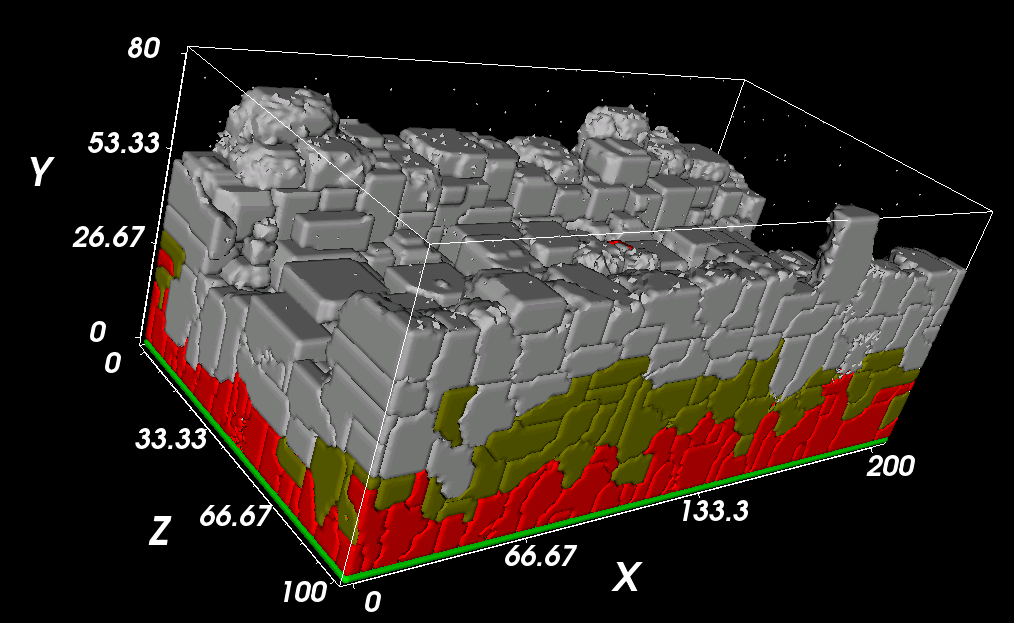
\includegraphics[width=12cm]{figures/SpaPcdbPcdiIn/MCS350000.png}
}
\end{center}
\begin{center}
\subfloat[]{
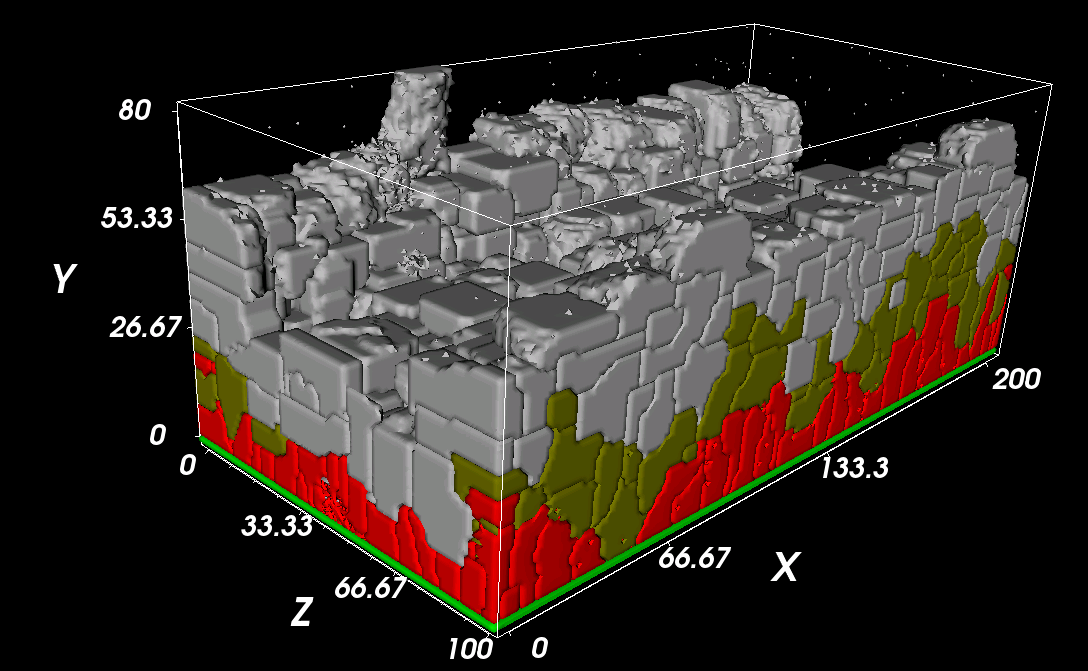
\includegraphics[width=12cm]{figures/SpaPcdbPcdiIn/MCS350000-1.png}
}
\end{center}
\caption[Simulated urothel with the model SPA/PCDB/PCDI at day 700]{\label{img:720daysScreenshotSPA/BCPD/IPCD}Screenshots at the end of an simulation of the model SPA/PCDB/PCDI, which lastet 700 days. Screenshot (a) is taken of an front view, whereas screenshot (b) is taken of the back of the urothelium.}

\end{figure}



